\chapter{Survey sulle tecniche di spam detection}
\lstset{basicstyle=\small\ttfamily,keywordstyle=\color{black}\bfseries,commentstyle=\color{darkgray},stringstyle=\color{black},showstringspaces=true}

Il capitolo illustra alcune tecniche di spam detection presenti in letteratura. Le tecniche verranno suddivise sulla base del tipo di segnali che vengono utilizzati: il contenuto, il grafo ed altri segnali (come ad esempio l'header delle richieste HTTP). Nella prima parte del capitolo verranno illustrate le tecniche basate sul contenuto, nella seconda parte le tecniche che fanno uso di grafi ed infine le tecniche che fanno uso di altri tipi di segnali.

\section{Tecniche basate sul contenuto}
\subsection{Prime feature per identificare lo spam}
\label{subsec:Feature}
Un metodo per identificare lo spam basandosi sul contenuto di una pagina web è quello di analizzare alcune proprietà (feature) delle pagine spam e confrontarle  con le medesime proprietà di quelle non spam al fine di ottenere dei valori con cui stimare la natura della pagina web (spam o non spam). Alcune di queste proprietà, come descritto in \cite{Fetterly:2004:SDS:1017074.1017077}, sono le seguenti:
\begin{itemize}
 \item 	\textit{Proprietà degli URL}: alcune analisi sulle proprietà dei link mostrano che gli URL di un host sono delle buone feature per identificare lo spam. In particolare l'URL di un host con molti caratteri, punti, slash e numeri è un buon indicatore di spam. Un modo semplice per classificare le pagine è quindi quello di usare un valore di soglia che definisca il numero massimo di tali caratteri per identificare una pagina come spam. 
 
 \item \textit{Host name resolution}: gli spammer possono popolare gli URL delle pagine spam con termini contenuti in query molto frequenti, che sono rilevanti per un certo settore,  e impostare un DNS per risolvere questi host name. Gli spammer cercano di manipolare il meccanismo  usato da alcuni motori di ricerca (ad esempio Google) che data una query \textit{q}, assegnano un rank più alto a un URL \textit{u} se i termini che compongono  il nome dell'host di \textit{u} combaciano con i termini della query. Perciò gli spammer creano tanti URL rilevanti per le diverse query in modo tale da far risultare la pagina di web spam tra i primi risultati di ricerca per molte query. Per determinare tale forma di spam, uno spam detector dovrebbe controllare quanti URL vengono risolti da uno stesso indirizzo IP.
 
 \item \textit{Proprietà del contenuto}: le pagine generate automaticamente hanno tutte lo stesso template, ad esempio numerosi siti di spam generano dinamicamente pagine con uno stesso numero di parole. Una tecnica per determinare lo spam è quella di clusterizzare le pagine in base alla somiglianza dei template. Considerando che le pagine di spam hanno strutture molto simili tra loro, se si identificano gruppi con molte pagine aventi la stessa struttura è probabile che esse siano spam.
\end{itemize}

Oltre a queste proprietà base, in \cite{Ntoulas:2006:DSW:1135777.1135794} vengono descritti ulteriori metodi e proprietà per l'individuazione dello spam. In tale studio i metodi e le proprietà descritti  sono il frutto di analisi effettuate dagli autori su un dataset di pagine HTML , che è stato ricavato utilizzando MSN Search crawler nell'agosto del 2004. Dalle analisi su tale dataset risulta che i domini con maggiore contenuto di spam sono: ``.biz'', ``.us'' e ``.com'' mentre le pagine contenenti più spam sono: francesi, tedesche e inglesi. I risultati sono rappresentati nei due grafici in figura \ref{fig:fetterly1} e in figura \ref{fig:fetterly2}. Nel primo grafico l'asse orizzontale rappresenta i domini e l'asse verticale mostra la frazione di spam all'interno di un dominio. I valori nel grafico sono riportati con un intervallo di confidenza del 95\% rappresentato dalla linea verticale sopra ogni barra. L'intervallo di confidenza varia in dimensione a causa del numero differente di campioni raffigurati 
nei deiversi domini. Nel secondo grafico l'asse orizzontale rappresenta la lingua della pagina e l'asse verticale rappresenta la frazione di spam per le pagine scritte in una particolare lingua. Anche nel secondo grafico i valori sono riportati con un intervallo di confidenza del 95\%.
\begin{figure}[htbp]
\centering
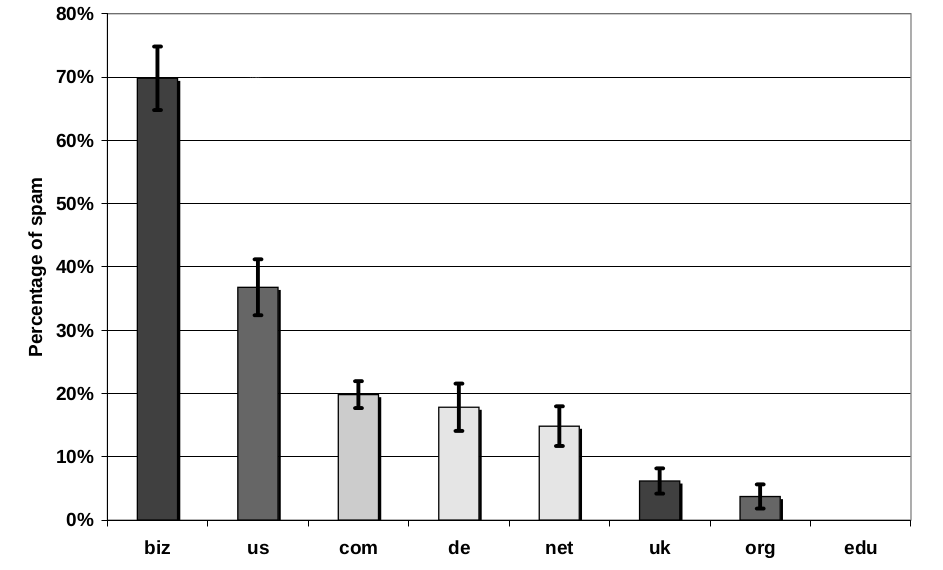
\includegraphics[width=12cm]{immagini/fetterly/fetterly1}
\caption{Occorrenze dello spam classificate per dominio all'interno del dataset descritto in \cite{Ntoulas:2006:DSW:1135777.1135794}}
\label{fig:fetterly1}
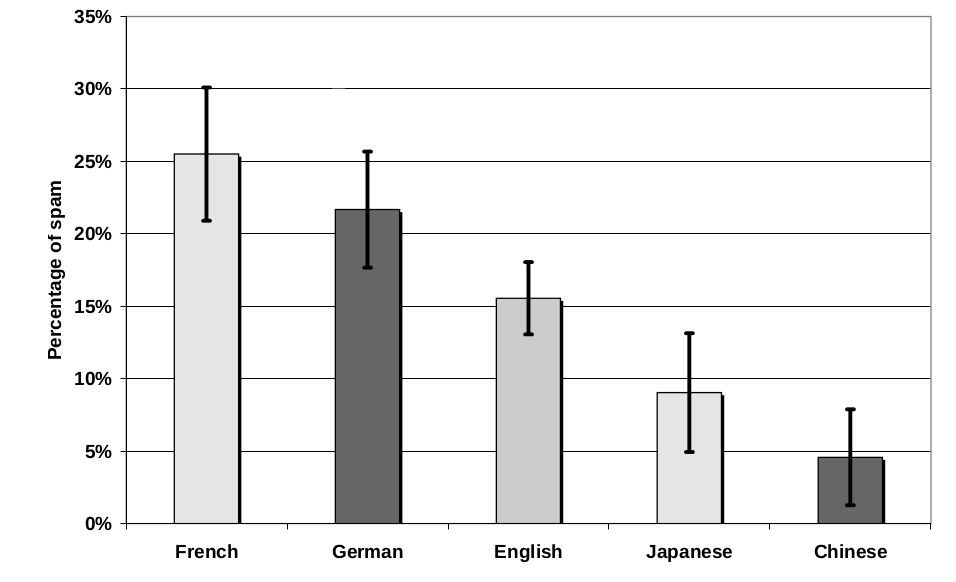
\includegraphics[width=12cm]{immagini/fetterly/fetterly2}
\caption{Occorrenze dello spam classificate per lingua all'interno del dataset descritto in \cite{Ntoulas:2006:DSW:1135777.1135794}}
\label{fig:fetterly2}
\end{figure}

Una proprietà che consente di identificare una pagina spam è il numero di parole all'interno della pagine stessa. Infatti una pratica molto comune nel costruire pagine spam è la cosiddetta ``Keyword stuffing'', un processo per cui al contenuto della pagina vengono aggiunte molte parole popolari che sono, tuttavia, irrilevanti  rispetto ai contenuti; lo scopo è di incrementare le probabilità della pagina di essere in cima ai risultati di molteplici query. In figura \ref{fig:fetterly3} viene plottato la distribuzione del numero di parole per ogni pagina del dataset (rappresentata dall'istogramma blu) correlata con la probabilità che una pagina sia spam (rappresentata dalla linea viola). Dal grafico si nota che la prevalenza di spam è più alta per le pagine contenenti molte parole. Perciò c'è una correlazione tra prevalenza di spam e numero di parole. Ma si può notare anche che il conteggio delle parole da solo non è una buona euristica visto che porta un alto tasso di falsi positivi.
\begin{figure}[htbp]
\centering
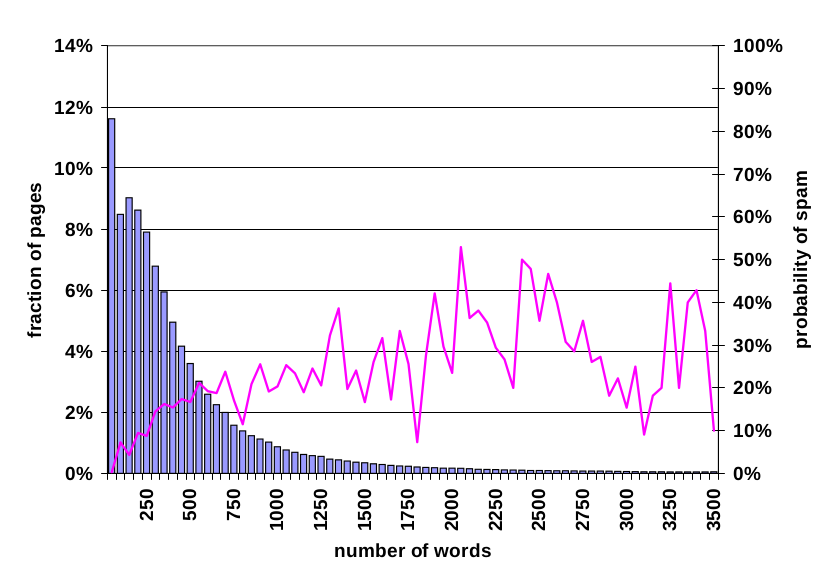
\includegraphics[width=12cm]{immagini/fetterly/fetterly3}
\caption{Prevalenza di spam sulla base del numero di parole per pagina}
\label{fig:fetterly3}
\end{figure}

La tecnica ``Keyword stuffing'' viene utilizzata anche per la scelta dei titoli, tenendo in considerazione che alcuni motori di ricerca assegnano un peso maggiore ai termini della query presenti all'interno del titolo della pagina. Il grafico in figura \ref{fig:fetterly4} rappresenta la distribuzione del numero di parole all'interno dei titoli delle pagine correlata con la probabilità che una pagina sia spam. Dal grafico si evince che un eccesso di parole all'interno del titolo è un indicatore di spam.
\begin{figure}[htbp]
\centering
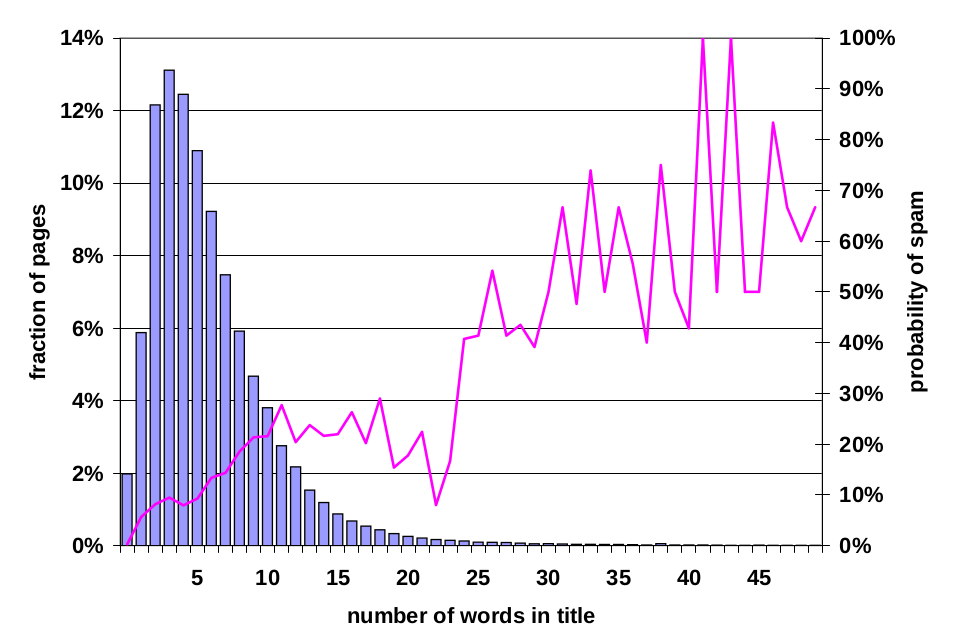
\includegraphics[width=12cm]{immagini/fetterly/fetterly4}
\caption{Prevalenza di spam sulla base del numero di parole all'interno dei titoli delle pagine}
\label{fig:fetterly4}
\end{figure}
Le parole che vengono utilizzate nel processo di ``keyword stuffing'' vengono selezionate casualmente o da un ristretto gruppo di query comuni. Per esaminare il comportamento con cui sono selezionate e costruite le frasi innanzitutto vengono identificate le \textit{n} parole più comuni all'interno del corpus; successivamente viene calcolata, per ogni pagina, la frazione delle parole comuni. Tale processo viene ripetuto per ogni scelta di \textit{n} (in figura \ref{fig:fetterly9} \textit{n=200}). Il grafico rappresenta la frazione di parole comuni per ogni pagina; esso ha una caratteristica gaussiana e suggerisce che la maggior parte delle pagine di spam sono generate tessendo parole da un dizionario con una scelta casuale.
\begin{figure}[htbp]
\centering
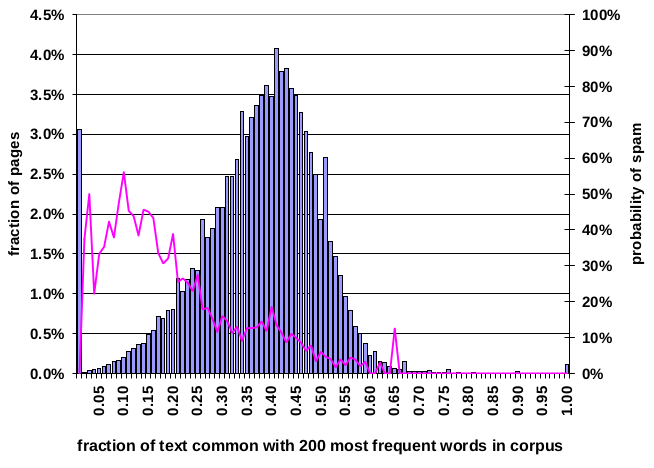
\includegraphics[width=12cm]{immagini/fetterly/fetterly9}
\caption{Prevalenza di spam sulla base della frazione di parole di una pagina che sono tra le 200 più frequenti parole nel corpus}
\label{fig:fetterly9}
\end{figure}
Un metodo che può essere adottato per identificare le pagine spam che sono generate automaticamente è descritto in \cite{Fetterly:2005:DPD:1076034.1076066}. 

Un altro dato utilizzato per determinare se una pagina è spam è la lunghezza media delle parole delle pagine. Dal dataset preso in considerazione in \cite{Ntoulas:2006:DSW:1135777.1135794} (grafico in figura \ref{fig:fetterly5}) si nota che la distribuzione della lunghezza media delle parole è simile a una gaussiana con moda e mediana corrispondenti a 5.0 e le parole con lunghezza media uguale a 10 sono certamente spam.
\begin{figure}[htbp]
\centering
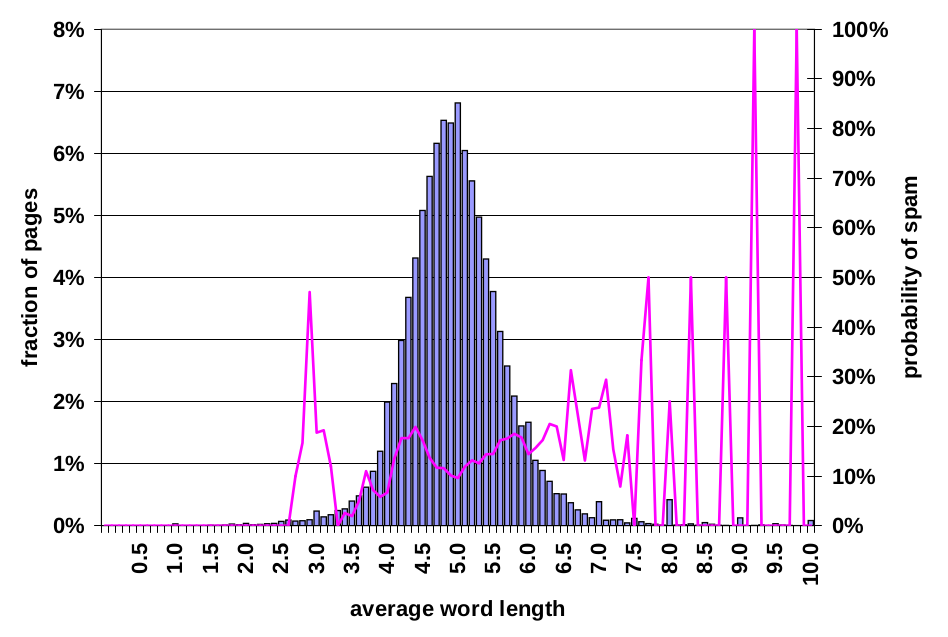
\includegraphics[width=12cm]{immagini/fetterly/fetterly5}
\caption{Prevalenza di spam sulla base della lunghezza media delle parole per pagina}
\label{fig:fetterly5}
\end{figure}

Un'altra proprietà delle pagine web che consente di stimare se una pagina è spam è la quantità di testo che è contenuta all'interno delle ancore (il tag ``\(<a>\)'' delle pagine web). Infatti una pratica comune dei motori di ricerca è considerare il testo delle ancore dei link in una pagina come annotazioni che descrivono il contenuto della pagina che viene puntata. L'idea principale è che se la pagina \textit{a} ha un link alla pagina \textit{b} con testo dell'ancora, ad esempio, ``computer'' allora potremmo concludere che \textit{b} parli di computer, anche se questa keyword non compare all'interno della pagina \textit{b}. Pertanto durante il ranking tali motori di ricerca potrebbero considerare la pagina \textit{b} come risultato di una query contenente la keyword ``computer''. Sfruttando questo meccanismo si creano pagine di spam contenenti solo del testo all'interno delle  ancore per valorizzare il ranking di altre pagine.; queste pagine di norma sono solo cataloghi di link ad altre pagine. Per 
capire meglio il fenomeno è stato calcolata la frazione di tutte le parole del testo delle ancore all'interno di una pagina, escludendo i markup rispetto al contenuto della pagina. In figura \ref{fig:fetterly6} viene visualizzato il grafico risultante. Si nota che un'alta frazione di testo delle ancore aumenta la probabilità che la pagina sia spam ma usare questa euristica da sola potrebbe portare un alto numero di falsi positivi \cite{Ntoulas:2006:DSW:1135777.1135794}.
\begin{figure}[htbp]
\centering
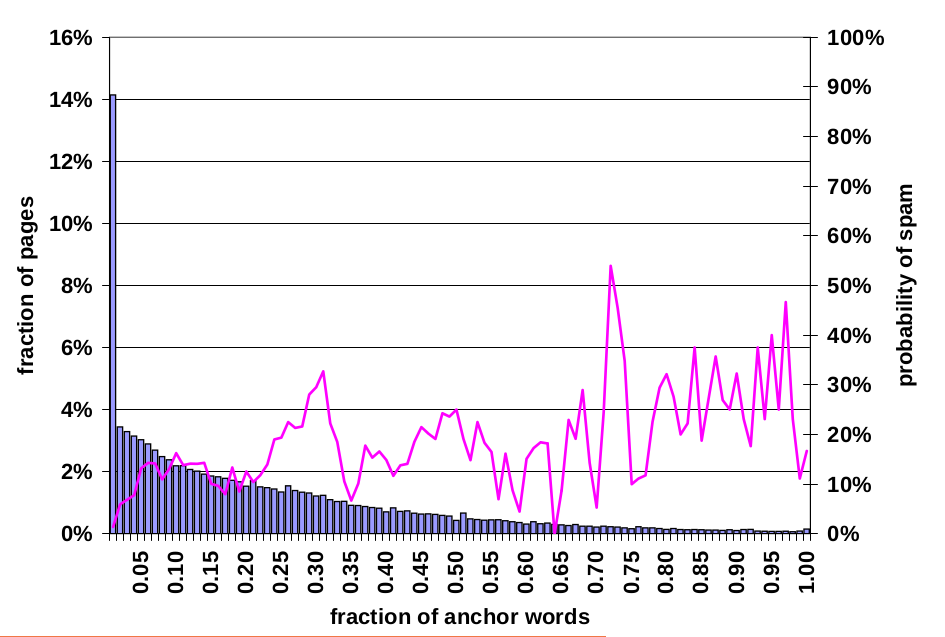
\includegraphics[width=12cm]{immagini/fetterly/fetterly6}
\caption{Prevalenza di spam sulla base della quantità di testo delle ancore delle pagine}
\label{fig:fetterly6}
\end{figure}

Calcolando la frazione di contenuto visibile all'interno di una pagina (definita come la lunghezza in termini di byte di tutte le parole non di markup) rispetto all'intera dimensione della pagina si nota dal grafico, in figura \ref{fig:fetterly7}, che la distribuzione (delle frazioni di contenuto visibile) evidenzia che le pagine di spam hanno meno markup delle pagine normali. Questo fa intendere che molte pagine spam hanno il solo scopo di dover essere indicizzate dai motori di ricerca  e non di essere fruite da un utente.
\begin{figure}[htbp]
\centering
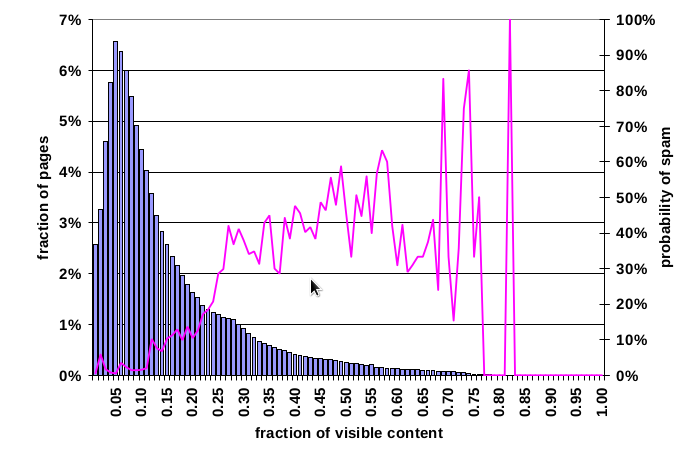
\includegraphics[width=12cm]{immagini/fetterly/fetterly7}
\caption{Prevalenza di spam sulla base della frazione di contenuto visibile}
\label{fig:fetterly7}
\end{figure}

Come detto in precedenza i  motori di ricerca possono dare un peso maggiore a pagine che contengono ripetutamente le keyword contenute nella query (ad esempio utilizzano come metodo di ranking il ``term-frequency''). Le pagine spam hanno, quindi,  contenuti replicati molte volte per aumentare il rank. Per rilevare la ridondanza di contenuti (ottenuta dal processo di replica), viene calcolato il rapporto di compressione ovvero la dimensione della pagina non compressa divisa per la dimensione della pagina compressa. In figura \ref{fig:fetterly8} è rappresentata la distribuzione del rapporto di compressione e la likelihood che la pagina sia spam. Dal grafico si nota che quanto più il valore di compressione è elevato tanto più probabilmente la pagina può essere considerata spam; il 70 per cento delle pagine con un rapporto di compressione maggiore di 4.0 sono giudicate spam. Questo è dovuto al fatto che una compressione su una pagina spam che ha contenuti ridondanti, sarà più efficace di una compressione su una 
pagina non spam che è caratterizza da contenuti non ridondanti. E perciò il rapporto di compressione tenderà a crescere quanto più la pagina sarà caratterizzata da contenuti ridondanti.
\begin{figure}[htbp]
\centering
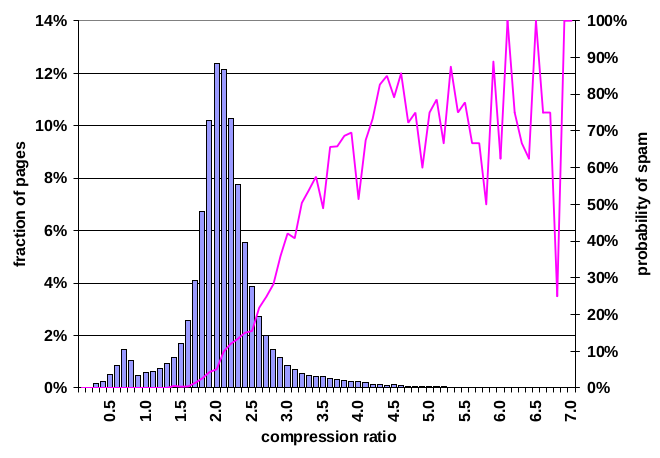
\includegraphics[width=12cm]{immagini/fetterly/fetterly8}
\caption{Prevalenza di spam sulla base del rapporto di compressione}
\label{fig:fetterly8}
\end{figure}

\subsection{Utilizzo di un classificatore per combinare le feature}
Sempre in \cite{Ntoulas:2006:DSW:1135777.1135794} le euristiche descritte fino a questo punto sono combinate considerando il problema di rilevamento dello spam come un problema di classificazione. Quindi  viene creato un classificatore, che usando le caratteristiche di una  pagina web la classificherà in una delle due classi: spam o non spam. Costruire un classificatore richiede una fase di training durante la quale i parametri del classificatore sono determinati e una fase di testing durante la quale le performance del classificatore sono valutate. Per ogni pagina all'interno del dataset viene calcolato il valore di ogni feature (ad esempio, usando le euristiche discusse sopra) e si utilizzano questi valori per istruire il classificatore. Il classificatore usato è un albero di decisione che dato un insieme di dati da traning e un insieme di feature crea un diagramma di flusso ad albero. Ogni nodo dell'albero corrisponde al test da valutare per una particolare feature mentre ogni arco è un valore di uscita 
del test 
ed 
infine le foglie corrispondono alle classi che verrano assegnate alle pagine. Un esempio del classificatore è rappresentato in figura \ref{fig:fetterly13}. Per migliorare il classificatore si possono usare tecniche come bagging o boosting. Queste tecniche creano un insieme di classificatori  che vengono combinati.
\begin{figure}[htbp]
\centering
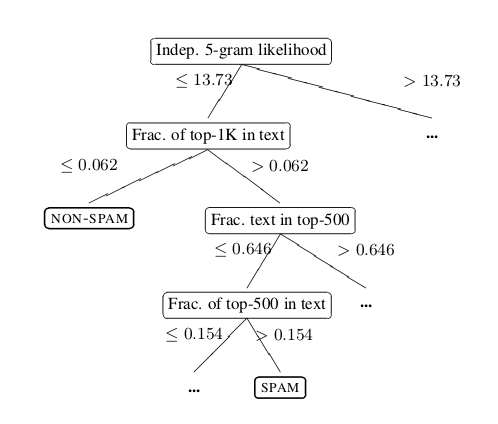
\includegraphics[width=8cm]{immagini/fetterly/fetterly13}
\caption{Esempio di classificatore}
\label{fig:fetterly13}
\end{figure}

\subsection{Language model per rilevare lo spam}
Oltre alle feature presentate in precedenza, in \cite{Martinez-Romo:2009:WSI:1531914.1531920} sono descritte nuove tipologie di feature e metodi per rilevare lo spam che fanno uso dei \textit{language model}  per analizzare le sorgenti estratte da ogni sito in un dataset. Le sorgenti sono dei pezzi di contenuto presenti all'interno delle pagine web di partenza (quelle che contengono i link ad altre pagine) e all'interno delle pagine web di destinazione (quelle che sono linkate dalle pagine di partenza). Per ogni sorgente si definisce un modello e si calcola quanto siano differenti i modelli individuati; viene utilizzata la \textit{Kullback-Leibler Divergence (KLD)} per misurare la divergenze tra le distribuzioni di probabilità dei termini di pagine web, applicandola a unità di testo della pagina di partenza e di quella linkata. La Kullback-Leibler (KL) è una misura  asimmetrica della divergenza che misura quanto male una distribuzione di probabilità \(M_q\) riesce a modellare \(M_d\):
\begin{equation}
KLD(T_1||T_2) = \sum_{t \in T_1} P_{T_1}(t) \log \frac{P_{T_1}(t)}{P_{T_2}(t)}
\label{eqn:kld}
\end{equation}
dove in \ref{eqn:kld} \(P_{T_1}(t)\) è la probabilità del termine \textit{t} nella prima unità di testo e \(P_{t_2}(t)\) è la probabilità del termine \textit{t} nella seconda unità di testo. In basso sono rappresentati due esempi di KLD applicata tra il testo delle ancore della pagina sorgente e i titoli delle pagine puntate dai link (esempio preso da WEBSPAM-UK2006). Dagli esempi si deduce che nel primo caso c'è una maggiore correlazione tra il testo dell'ancora della pagina sorgente e il titolo della pagina puntata rispetto al secondo esempio dove il valore di KLD e maggiore.
\begin{lstlisting}[frame=trbl,postbreak=\space, breakindent=5pt, breaklines]
KLD(Free Ringtones || Free Ringtones for Your Mobile Phone from PremieRingtones.com) = 0.25

KLD(Best UK Reviews || Findabmw.co.uk - BMW Information Resource) = 3.89
\end{lstlisting}
Per determinare se una pagina è spam si cerca di identificare una relazione tra due pagine collegate sulla base del valore di divergenza. I valori sono ottenuti calcolando le divergenze con KLD tra una o più sorgenti di informazioni da ogni pagina. In particolare si usano tre tipi di informazione di una pagina sorgente: testo delle ancore, testo intorno alle ancore, termini nell'URL mentre per la pagina che viene linkata dalla pagina sorgente: titolo, contenuto della pagina e meta tag. Combinando queste sorgenti di informazione si determina la divergenza tra due pagine; di seguito vengono descritte alcune combinazioni base:
\begin{itemize}
\item testo delle ancore - contenuto. Una pagina che ha un link verso un'altra pagina ha solo un modo per convincere l'utente a visitare la pagina collegata: mostrare in maniera concisa le informazioni relative alla pagina collegata. Perciò una grande divergenza tra questi due frammenti di testo indica che la pagina può essere spam. In figura \ref{fig:martinez1} è illustrata la divergenza KL tra le due sorgenti di informazione, come si vede la curva delle pagine normali è più compatta di quella delle pagine spam.
\begin{figure}[htbp]
\centering
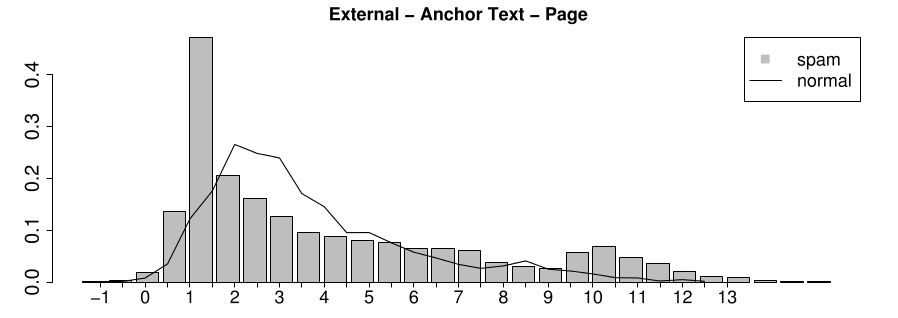
\includegraphics[width=12cm]{immagini/martinez/martinez1}
\caption{Istogramma della divergenza KL tra testo delle ancore e il contenuto della pagina puntata basato sul dataset WEBSPAM-UK2006 utilizzato in \cite{Martinez-Romo:2009:WSI:1531914.1531920}}
\label{fig:martinez1}
\end{figure}

\item testo vicino alle ancore - contenuto. Il testo delle ancore, a volte, è un valore poco descrittivo e per ovviare al problema viene usato il testo che circonda le ancore. Nell'esperimento vengono utilizzate 7 parole per lato. In figura \ref{fig:martinez2} viene mostrato che le pagine spam hanno alti valori di divergenza mentre le normali sono concentrate intorno \(KL \approx  2.5\), .
\begin{figure}[htbp]
\centering
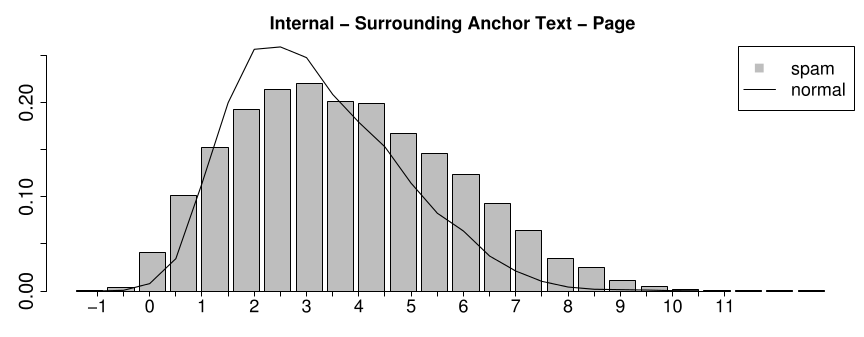
\includegraphics[width=12cm]{immagini/martinez/martinez2}
\caption{Istogramma della divergenza KL tra testo intorno alle ancore e il contenuto della pagina puntata basato sul dataset WEBSPAM-UK2006 utilizzato in \cite{Martinez-Romo:2009:WSI:1531914.1531920}}
\label{fig:martinez2}
\end{figure}

\item termini nell'URL - contenuto. I motori di ricerca danno molta importanza agli URL perché i termini che  li compongono  possono dare un'idea del contenuto della pagina a cui l'URL fa riferimento.  Un metodo di spam che sfrutta questo meccanismo consiste nella creazione di URL contenenti molti termini comuni (ad esempio: \url{www.domain.com/viagra-youtube-free-download-poker-online.html} che in realtà è solo uno store online e non ha alcuna attinenza con i nessuno dei termini utilizzati nell'URL). Al fine di identificare questo tipo di spam, vengono prelevati i termini più rilevanti da un URL e calcolata la divergenza col contenuto della pagina di destinazione. La distribuzione finale, rappresentata in figura \ref{fig:martinez3}, dimostra una grande differenza tra l'istogramma delle pagine normali con quello delle pagine spam.
\begin{figure}[htbp]
\centering
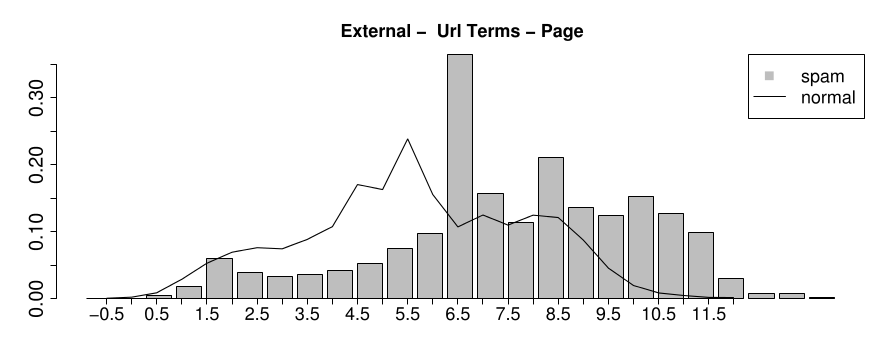
\includegraphics[width=12cm]{immagini/martinez/martinez3}
\caption{Istogramma della divergenza KL tra termini degli URL e il contenuto della pagina puntata basato sul dataset WEBSPAM-UK2007 utilizzato in \cite{Martinez-Romo:2009:WSI:1531914.1531920}}
\label{fig:martinez3}
\end{figure}

\item testo delle ancore - titolo. Questa feature si compone di due sorgenti che sono molto simili in quanto descrivono la pagina con poche parole. Tuttavia la prima sorgente può essere scritta anche da chi non è il proprietario della pagina di destinazione.  In figura \ref{fig:martinez4} notiamo che questa feature da sola non discrimina bene le pagine spam ma è abbastanza efficace se utilizzata in congiunzione con altre feature.
\begin{figure}[htbp]
\centering
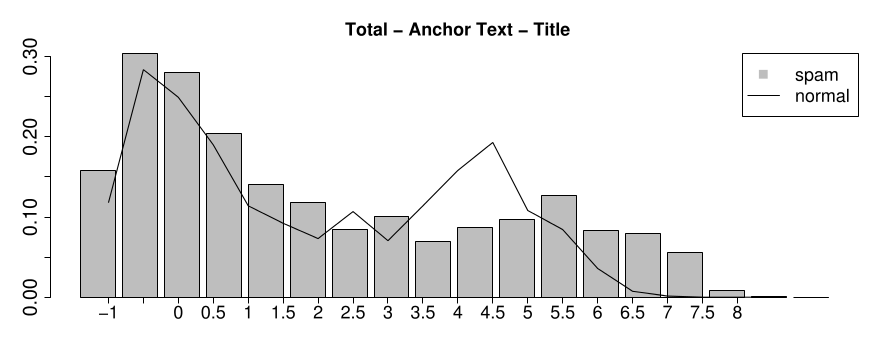
\includegraphics[width=12cm]{immagini/martinez/martinez4}
\caption{Istogramma della divergenza KL tra testo delle ancore e titolo della pagina puntata basato sul dataset WEBSPAM-UK2007 utilizzato in \cite{Martinez-Romo:2009:WSI:1531914.1531920}}
\label{fig:martinez4}
\end{figure}

\item testo intorno alle ancore - titolo. Dal grafico in figura \ref{fig:martinez5} si può notare come tale feature rileva meglio lo spam rispetto alla precedente, infatti molti valori di spam sono concentrati per valori di \(KL > 3\).
\begin{figure}[htbp]
\centering
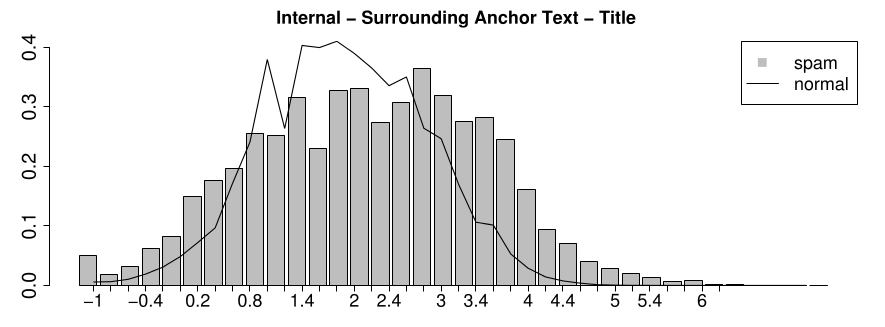
\includegraphics[width=12cm]{immagini/martinez/martinez5}
\caption{Istogramma della divergenza KL tra testo intorno alle ancore e titolo della pagina puntata basato sul dataset WEBSPAM-UK2006 utilizzato in \cite{Martinez-Romo:2009:WSI:1531914.1531920}}
\label{fig:martinez5}
\end{figure}

\item termini nell'URL - titolo. In questa feature entrambe le sorgenti sono generate dal proprietario della pagina, a differenza della precedente in cui la sorgente di  informazione della pagina di partenza poteva essere generata da un'altra persona. In questo vi dovrebbe essere maggiore coerenza tra le due sorgenti. In figura \ref{fig:martinez6} sono rappresentate le distribuzioni per le pagine spam e non spam.
\begin{figure}[htbp]
\centering
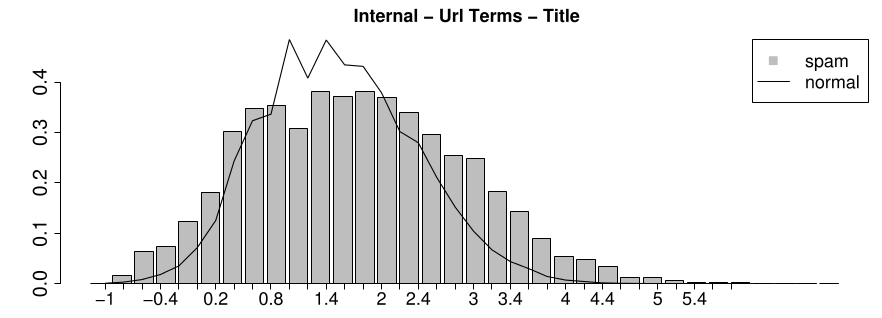
\includegraphics[width=12cm]{immagini/martinez/martinez6}
\caption{Istogramma della divergenza KL tra termini nell'URL e titolo della pagina puntata basato sul dataset WEBSPAM-UK2006 utilizzato in \cite{Martinez-Romo:2009:WSI:1531914.1531920}}
\label{fig:martinez6}
\end{figure}

\item titolo - contenuto. I motori di ricerca danno un peso maggiore ai termini della query se presenti nel titolo della pagina. Sfruttando tale meccanismo gli spammer perfezionano i loro processi in modo tale da impostare termini chiave nel titolo anche creando però una divergenza tra titolo e contenuto della pagina. La feature titolo - contenuto consente la rilevazione di spam quando non vi è alcuna relazione tra il titolo e il contenuto della pagina. In figura \ref{fig:martinez7} è rappresentata la divergenza tra le due distribuzioni spam e non spam. 
\begin{figure}[htbp]
\centering
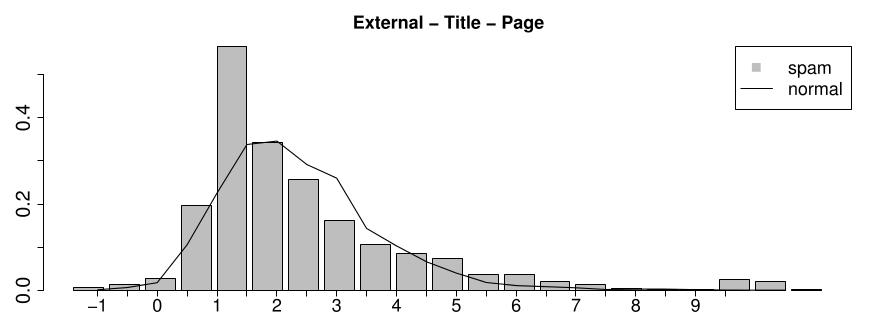
\includegraphics[width=12cm]{immagini/martinez/martinez7}
\caption{Istogramma della divergenza KL tra titolo  e contenuto della pagina basato sul dataset WEBSPAM-UK2006 utilizzato in \cite{Martinez-Romo:2009:WSI:1531914.1531920}}
\label{fig:martinez7}
\end{figure}

\item metatag. Vengono usati per calcolarne la divergenza con altre sorgenti di informazioni della pagina di partenza (come il testo delle ancore e il testo intorno alle ancore) e della pagina destinazione (come il contenuto o i temini dell'URL). In figura \ref{fig:martinez8} viene visualizzata la divergenza tra il testo delle ancore e i metatag.
\begin{figure}[htbp]
\centering
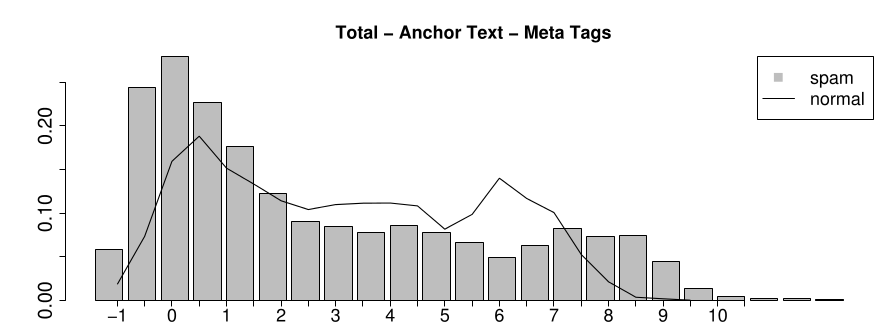
\includegraphics[width=12cm]{immagini/martinez/martinez8}
\caption{Istogramma della divergenza KL tra testo delle ancore  e i meta tag della pagina basato sul dataset WEBSPAM-UK2006 utilizzato in \cite{Martinez-Romo:2009:WSI:1531914.1531920}}
\label{fig:martinez8}
\end{figure}
\end{itemize}
Oltre alle feature descritte si possono ottenere delle feature più articolate combinando le feature base tra di loro; ad esempio per le pagine sorgenti si possono definire: testo delle ancore e termini nell'URL , testo intorno alle ancore e URL (per maggiori dettagli \cite{Martinez-Romo:2009:WSI:1531914.1531920}).

Infine tali feature possono essere usate per istruire un classificatore.

\subsection{Spam detection sulla base degli argomenti di una pagina web}
Dong et al. \cite{Dong:2012:EDC:2457524.2457693} propongono un metodo basato su statistiche effettuate sugli argomenti delle pagine. Le statistiche non si basano sulle parole della pagina ma sugli argomenti, in modo da non ignorare la semantica delle parole e di catturare le feature linguistiche nascoste nel testo per capire se la pagina è spam. Le analisi vengono fatte usando i topic model, modelli statistici che scoprono gli argomenti latenti presenti in una collezione di documenti. Un topic model utilizzato è la \textit{Latent Dirichlet Allocation (LDA)} che modella ogni argomento latente come una distribuzione probabilistica su un vocabolario e ogni documento come una distribuzione probabilistica sugli argomenti latenti. L'intuizione di usare i topic model per analizzare il contenuto  delle pagine web nasce dal fatto che analizzando le feature nascoste di una pagina spam, gli autori hanno notato che i contenuti di queste pagine, generati automaticamente, sono differenti dai contenuti delle pagine non 
spam. Vengono definiti tre tipi di misure.

La prima misura per determinare le pagine spam utilizzando LDA sfrutta la caratteristica che tali pagine sono molto topic-centric, ovvero hanno uno specifico insieme di argomenti. In figura \ref{fig:zhou1} sono rappresentate quattro distribuzioni degli argomenti presenti in quattro pagine (due spam e due non spam) scelte casualmente da un dataset. A supporto della tesi degli autori che le pagine spam sono topic centric si può notare che presentano una distribuzione esponenziale, in quanto esse vengono sviluppate per avere un alto ranking per un insieme di  specifiche query di ricerca, al contrario delle pagine non spam che presentano una distribuzione uniforme (nell'articolo gli autori sostengono che le pagine non spam come una homepage contengono vari argomenti come ad esempio: i contatti, chi e cosa fa, altre informazioni).
\begin{figure}
\centering
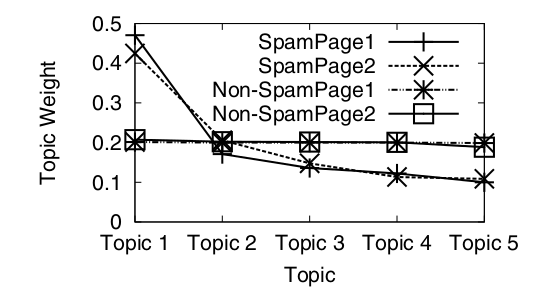
\includegraphics[width=10cm]{immagini/zhou/immagine1.png}
\caption{Distribuzione degli argomenti pesati per pagine spam e normali}
\label{fig:zhou1}
\end{figure}
Per classificare le pagine sulla base di questa caratteristica, basata sulle distribuzioni degli argomenti, è stato proposto una misura della  diversità degli argomenti basata sulla varianza. Data una pagina web \(d\), la sua distribuzione degli argomenti è \(T(d)=\{t_1,t_2,......,t_m\}\), dove ogni argomento \(t_i (1 \leq i \leq m)\) è associato con un peso \(\delta_{t_i}\). La misura della diversità degli argomenti basata sulla varianza per \(d\), denotata con \(TopicVar(d)\), è calcolata come:
\begin{equation}
TopicVar(d)=\frac{\sum_{i=1}^m (\delta_{t_i}-u)^2}{m}
\end{equation}
dove \(u=\frac{\sum_{i=1}^m\delta{t_i}}{m}=\frac{1}{m}\).
In figura \ref{fig:zhou2} è illustrata la distribuzione risultante. Dalla distribuzione si nota che le pagine spam sono più topic-centric ovvero la varianza dei pesi degli argomenti è piu grande rispetto alle pagine non spam. Questo è dovuto al fatto che le pagine non spam avendo una distribuzione quasi uniforme hanno una la varianza che è più piccola rispetto alle pagine spam che hanno una distribuzione più concentrata di quella uniforme, come quella esponenziale. Il valore di \textit{TopicVar} è proporzionale alla probabilità che una pagina sia spam, ovvero all'aumento della probabilità di una pagina di essere spam consegue un aumento del valore di \textit{TopicVar} per quella pagina. Questa misura è un ottimo indicatore per rilevare lo spam.
\begin{figure}
\centering
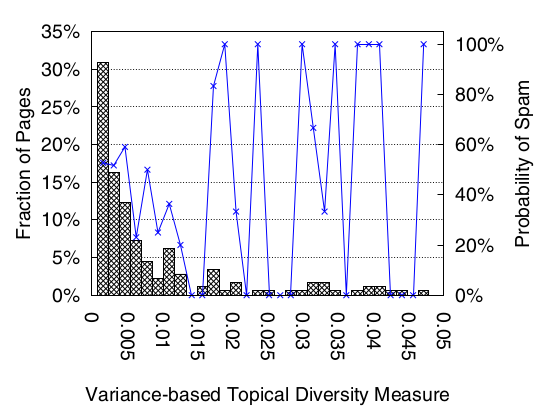
\includegraphics[width=10cm]{immagini/zhou/immagine2.png}
\caption{Prevalenza di spam relativa alla misura della  diversità degli argomenti basata sulla varianza }
\label{fig:zhou2}
\end{figure}

La seconda misura per identificare le pagine spam utilizzando LDA che permette di misurare la relazione semantica tra gli argomenti è  la semantica delle parole. Gli autori definiscono che: data una pagina web \(d\), la sua distribuzione degli argomenti è \(T(d)=\{t_1,t_2,........,t_m\}\). La probabilità che un parola \(w\) appartenga a un argomento \(t_i (1 \leq i \leq m )\) è definita come \(\phi(w|t_i)\). Ogni argomento \(t_i\) è rappresentato come un insieme di parole denotate come \(W(t_i)\). Intuitivamente due argomenti \(t_i, t_j (1 \leq i, j \leq m)\) sono semanticamente correlati se le parole \(W(t_i)\) e \(W(t_j)\) sono semanticamente legate. In \cite{Dong:2012:EDC:2457524.2457693} per ottenere le relazioni semantiche tra le due parole è utilizzata una funzione di similarità \(Sim(w_i,w_j)\) che è quella di Wordnet. Quindi per misurare la relazione semantica tra due argomenti \(t_i,t_j\), si calcolano le similarità tra ogni coppia di parole dei due argomenti moltiplicate con le loro probabilità 
rispetto agli argomenti.
\begin{equation}
\label{eqn:1}
Sim(t_i,t_j) = \frac{\sum_{w_k \in W(t_i),w_l \in W(t_j)}Sim(w_k,w_l) X \phi(w_k|t_i) X \phi(w_l|t_j)}{\frac{|W(t_i)| X |W(t_j)|}{2}}	
\end{equation}
Usando quindi un modello degli argomenti otteniamo \(m\) argomenti latenti. Dall'equazione \ref{eqn:1} si deriva una misura della diversità degli argomenti basata sulla semantica per gli \(m\) argomenti latenti di una collezione \cite{Dong:2012:EDC:2457524.2457693}: data una pagina web \(d\), la sua distribuzione degli argomenti è \(T(d)\) e quindi la misura della diversità degli argomenti basata sulla semantica per tale pagina \(d\) è:
\begin{equation}
TopicSim(d)=\frac{\sum_{1 \leq i \leq j \leq m} Sim(t_i,t_j)}{\frac{1}{2} m(m-1)}
\end{equation}
In figura \ref{fig:zhou3} è illustrata la distribuzione della misura di diversità degli argomenti basata sulla semantica.
\begin{figure}
\centering
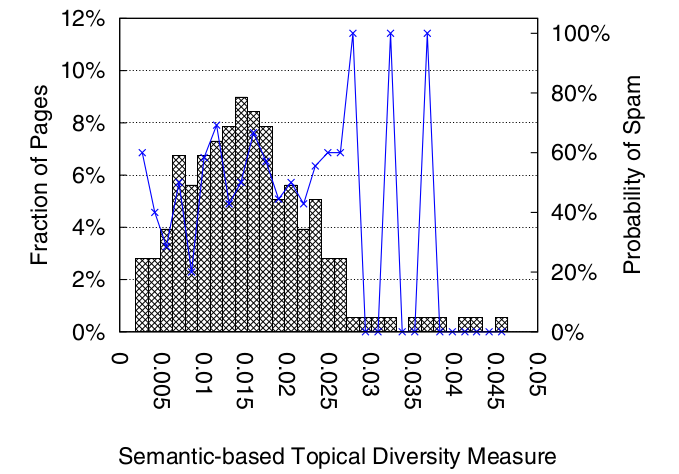
\includegraphics[width=10cm]{immagini/zhou/immagine3}
\caption{Prevalenza di spam relativa alla misura di diversità degli argomenti basata sulla semantica}
\label{fig:zhou3}
\end{figure}
Dalla distribuzione si nota che quando la misura cresce la probabilità che una pagina sia spam aumenta, ovvero le pagine spam hanno argomenti che sono in forte relazione semantica tra loro e cioè sono icentrate su pochi argomenti.

L'ultima misura è basata sulla massima semantica ed è definita come:
\begin{equation}
TopicSimMax(d)= max\{Sim(t_i,t_j)|1 \leq i \leq j \leq m \}
\end{equation}
La distribuzione della misura di diversità basata sulla massima semantica mostra che questa è più alta per le pagine che contengono spam. La distribuzione è rappresentata in figura \ref{fig:zhou4}.
\begin{figure}	
\centering
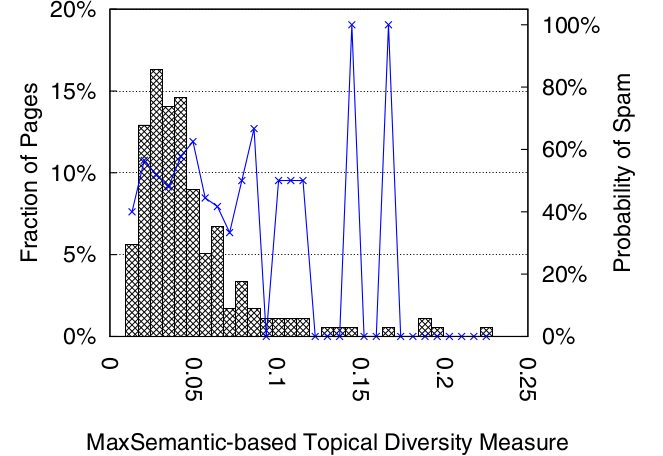
\includegraphics[width=10cm]{immagini/zhou/immagine4}
\caption{Prevalenza di spam relativa alla misura di diversità sulla massima semantica}
\label{fig:zhou4}
\end{figure}

Anche in questo caso per determinare se una pagina è spam oppure non spam, vengono utilizzati algoritmi supervisionati di apprendimento per istruire un classificatore di pagine spam usando misure di diversità degli argomenti. Con LDA possiamo impostare parametri come il numero di argomenti e il numero di parole per ogni argomento che incidono sulle le prestazioni della classificazione.

\subsection{Altre tecniche}
Nello studio in \cite{Abernethy:2008:WSI:1451983.1451994} viene presentato  l'algoritmo WITCH (Web Spam Identification Through Content and Hyperlinks), un algoritmo ibrido che utilizza sia il contenuto della pagina che la struttura dei link per identificare le pagine spam. Come descritto in precedenza nel sotto capitolo \ref{subsec:Feature}, le differenti proprietà tra le pagine spam e non spam possono essere sfruttate per costruire un classificatore. Per identificare lo spam l'algoritmo WITCH  utilizza le feature descritte in precedenza e analizza la struttura dei collegamenti tra le pagine. In particolare viene istruito un classificatore lineare nello spazio delle feature usando la SVM (Support Vector Machine) come funzione obbiettivo. I collegamenti tra le pagine sono utilizzati in modo da regolarizzare il grafo, che produce una predizione che varia leggermente tra le pagine dei link. Il metodo SVM associato alla regolarizzazione del grafo è efficiente per il rilevamento di web spam. 

Un altro metodo, proposto in \cite{DBLP:conf:airweb:UrvoyLF06}, è denominato ``Hidden style similarìty measure'' ed è basato su feature extra testuali appartenenti alle pagina HTML. Infatti gli autori sostengono che le pagine spam generate automaticamente non sono facili da rilevare utilizzando metodi classici di classificazione basati solamente sul contenuto; gli autori quindi utilizzano la struttura HTML di una pagina per classificare le pagine simili.

\section{Tecniche basate sul grafo}
Tali tecniche fanno uso del grafo del web ricavato dai collegamenti ipertesuali tra le pagine. Il web, quindi, può essere rappresentato come un grafo diretto \textit{G = (V,E)}, dove \textit{V} è l'insieme delle pagine e rappresentano i nodi del grafo mentre \textit{E} è l'insieme dei link diretti tra le pagine. Il grafo può essere astratto e rappresentato da una matrice di transizione cosi formata:
\begin{equation}
T(p,q)=\left \{
\begin{array}{cc}
0 & if(q,p) \in E\\
1/\omega(q) & if(q,p) \in E
\end{array}
\right .
\end{equation}
dove \(\omega(p)\) è il grado di link in uscita della pagina \(p\).
Possiamo anche definire la matrice di transizione inversa U:
\begin{equation}
U(p,q)=\left \{
\begin{array}{cc}
0 & if(p,q) \in E\\
1/l(q) & if(p,q) \in E
\end{array}
\right .
\end{equation}
dove \(l(q)\) è il grado di link in ingresso della pagina \(q\).
\subsection{Metodi classici per identificare lo spam web usando il grafo}
Uno dei primi metodi adottati per identifiare lo spam web usando il grafo è \textit{Trustrank} \cite{Gyongyi:2004:CWS:1316689.1316740}. \textit{Trustrank} fa uso di un insieme di pagine di partenza \(S\) che sono valutate da degli esperti e che vengono classificate in due sottoinsiemi: pagine non spam \(S^+\) e pagine spam \(S^-\); questo fase è chiamata funzione \textit{Oracle}. Per determinare le pagine non spam senza invocare la funzione \textit{Oracle} su tutto il grafo derivato dalla fase di crawling, viene fatta un'assunzione empirica chiamata \textit{isolazione approssimata dell'insieme delle pagine buone} la quale afferma che le pagine non spam raramente punteranno a quelle spam perché gli sviluppatori di pagine non spam hanno poco interesse nel linkare pagine spam almeno che non vengano ingannati tramite ad esempio l'uso di tecniche come l'\textit{honeypot}. Dato un numerto limitato di chiamate della funzione \textit{Oracle} sul seed set di partenza e sfuttando l'assunzione fatta precendentemente 
viene definita una funzione, denominata come \textit{funzione di verità ignorante \(T_0\)}, per ogni pagina pagina \(p\) del grafo:
\begin{equation}
T_0(p)=\left\{
\begin{array}{ccc}
O(p) & if & p\in S \\
1/2 & altrimenti
\end{array}
\right .
\end{equation}
dove la funzione \(O\) è la funzione \textit{Oracle}. Dal momento che le pagine buone dovrebbero puntare ad altre pagine buone assegnamo 1 a tutte le pagine che possono essere raggiunte da una pagina in \(S^+\) in \(M\) step. La funzione di verità \(T_M\) è definita come:
\begin{equation}
T_M(p)=\left\{
\begin{array}{ccccc}
O(p) & if & p\in S \\
1 & if & p \not\in S & and & \exists q\in S^+:q\rightarrow_M p \\
1/2 & altrimenti
\end{array}
\right .
\end{equation}
Il percorso  dalla pagina \(q\) a \(p\) nell'equazione non comprende pagine spam incluse nell'insieme \(S^-\).

Il problema della funzione di verità \(T_M\) è che non esiste la sicurezza che le pagine raggiungibili da pagine buone siano effetivamente della stessa carattesistica. Infatti più lontana una pagina \(p\) si trova dal seed set \(S^+\) minore è la certezza che quella pagina sia buona. Un modo per non incorrere in questo errore è ridurre il valore della funzione di verità ogni qual volta ci si allontana dal seed set \(S^+\).

In figura \ref{fig:trustrank1} è possibile vedere in dettaglio l'algoritmo. L'algoritmo calcola il valore di verità di ogni pagina dell'intero grafo. I valori di input sono il grafo descritto dalla matrice di transizione \(T\) e il numero di pagine \(N\) e i parametri di controllo dell'esecuzione: \(L\) il numero di chiamate della funzione \(Oracle\) e \(\alpha_b\) il fattore di decadimento per il calcolo di \textit{Pagerank} ed infine \(M_b\) il numero di iterazioni per il calcolo di \textit{Pagerank}. Al primo passo viene invocata la funzione \textit{SelectSeed()} calcola l'insieme delle pagine con il relativo rank di rilevanza per essere incluse nel seedset di partenza. Nel secondo punto la funzione \(Rank(x,s)\) ordina gli elementi di \(x\) in modo decrescente sulla base dello score di \(s\). Il punto tre invoca la funzione \textit{Oracle} su \(L\) pagine. I valori del vettore \(d\) che corrispondono alle pagine buone del seed sono imposate a 1. Nel punto (4) il vettore viene normalizzato in modo tale 
che la somma faccia 1. Infine al punto (5) viene calcolato \textit{Trustrank} usando \textit{Pagerank} personalizzato dal vettore \(d\) che rimpiazza la distribuzione uniforme. Dall'algoritmo si nota che \textit{Trustrank} è una versione modificata di \textit{Pagerank} dove il vettore di teletrasporto è il seed set \(S^+\) calcolato al punto 3 e 4.
\begin{figure}
\centering
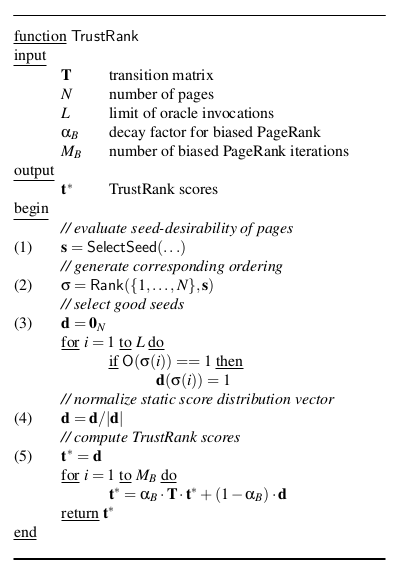
\includegraphics[width=8cm]{immagini/trustrank/trustrank}
\caption{Algoritmo di trustrank}
\label{fig:trustrank1}
\end{figure}

Un altro algoritmo che è stato progettato per identificare lo spam usando come input il grafo delle pagine web è \textit{Anti-Trust Rank} \cite{Krishnan06webspam}. Questo algoritmo sfrutta la stessa intuizione di \textit{Trustrank} dell'isolamento approssimato cioè che pagine buone molto raramente punteranno a pagine malevoli;  quindi si popola un seed set formato da pagine spam e si propaga la funzione Anti Trust (che sarebbe la funzione di verità di Trustrank) sul grafo trasposto con l’obbiettivo di rilevare le pagine spam, le quali successivamente possono essere filtrate da un motore di ricerca. Più precisamente a differenza per quanto avviene in \textit{Trustrank} dove la funzione \textit{Trust} è propagata dal seed set composto da pagine non spam lungo tutto il grafo, in \textit{Anti-Trust Rank} la funzione (in questo caso la funzione \textit{Anti Trust}) è propagata nella direzione inversa ai link in entrata ad ogni pagina del grafo, partendo da un insieme di pagine del seed set composto da pagine spam.
 L'obbiettivo è assegnare un rank maggiore alle pagine spam e successivamente eliminarle dalle ricerche o usando un valore di soglia oppure ritornando le \(n\) pagine che hanno valore di \textit{Anti-Trust Rank} più alto.
 
\textit{Trustrank} e \textit{Anti-Trust rank} sono ottimi algoritmi per identificare lo spam, ma hanno il problema che l’insieme seed usato potrebbe non essere sufficientemente rappresentativo per coprire bene tutti gli argomenti del web. Un modo naturale di ottenere una grande copertura del web è usare gli argomenti delle pagine come segnale di ingresso: invece di usare un singolo valore di \textit{trustrank} per un sito, in \cite{Wu:2006:TTU:1135777.1135792} gli autori propongono di calcolare \textit{trustrank} per i differenti argomenti di ogni sito. L'algoritmo consiste nel partizonare il seed set sulla base dei vari argoementi che esso contiene e usare ognuna di queste partizioni come seed set per calcolato il valore di \textit{trustrank} per ogni pagina.

Un altro metodo per l'identificazione di pagine spam è descritto in \cite{Caverlee:2007:CWS:1281100.1281124}. Questo metodo separa la credibilità di una pagina dalla credibilità del link per quella pagina al contrario di \textit{pagerank} che è manipolabile tramite tecniche come \textit{hoenypot}. La credibilità viene definita in termini di credibilità \textit{k-scope}. Data una funzione \(C\) essere una funzione di credibilità che istantaneamente valuta la qualità di un link di un pagina \(p\) al tempo \(t\), un valore di \(C(p,t)=0\) indica che \(p\) non è credibile mentre \(C(p,t)=1\) indica che \(p\) è credibile. Dato  un percorso in un grafo diretto \(G\) dalla pagina \(p\) alla pagina \(q\) essere la sequenza di nodi: \(path(p,q)=(n_0,n_1,...,n_j)\) dove \(p=n_0, q=n_j\) tale che esiste un arco diretto tra nodi successivi nel percorso \(n_i,n_{i+1}\in L\) per \(0\leq i \leq j-1\), diciamo che un percorso  in un grafo diretto \(G\) dalla pagina \(p\) alla pagina \(q\) è un \textit{bad path} se la pagina di destinazione è una pagina spam \(q\in P_b\) (dove \(P_b\) è l'insieme delle pagine spam) e nessuna altra pagina nel percorso è una pagina spam. \(path(p,q)=(n_0,n_1,...,n_j)\) e \(q\in P_b\) e \(n_i\not\in P_b (0\leq i\leq j-1)\). La probabilità che una camminata casuale passi, lungo un percorso di lunghezza \(k\), da una pagina \(p\) è denotata con \(Pr(path_k(p))\) ed è determinata con i pesi degli archi per ogni hop nel percorso:
\begin{equation}
 PR(path_k(p))=\prod_{i=0}^{k-1}w(n,n_{i+1})
\end{equation}
Quindi credibilità \textit{k-scope} di una pagina  è definita in termini di probabilità che una camminata casuale eviti le pagine spam dopo aver superato \(k\) hop dalla pagina di origine. La credibilità \textit{k-scope} di una pagina \(p\) al tempo \(t\), denotata con \(C_k(p,t)\) è definita come segue:
\begin{equation}
 C_k(p,t)=1-\sum_{l=1}^k\left (\sum_{path_l(p)\in BPath_l(p)}Pr(path_l(p))\right )
\end{equation}
Nel caso \(p\in P_b\) allora \(C_k(p,t)=0\). Nel caso in cui non ci siano pagine spam all'interno di \(k\) hop di pagine allora \(p\) è credibile con un valore \(C_k(p,t)=1\) se lei è un pagina spam o nel caso in cui tutti i percorsi originati da \(p\) colpiscono una pagina \(p\) all'intenro di \(k\) hop, allora \(p\) no è credibile \(C_k(p,t)=0\). Ma dato che non che non è possibile avere tutto il grafo e non c'è nessuna sicurezza sulla conoscenza totale dei nodi spam è stato introdotto il concetto di cerdibilità tunable k-Scope, la quale aumenta il calcolo della credibilità k-scope includendo un fattore di penalità di credibilità. GLi obbiettivi sono approssimare al meglio la credibilità k-scope sotto limiti reali e capire come parametri differenti protrebbero influire sulla qualità delle varie funzioni usate. Sia \(G=(P,L)\) essere un grafo diretto, k il raggio massimo di camminata e \(\gamma(p)\) il fattore di penalità di credibilità di una pagina \(p\in P\) dove \(0\leq \gamma(p)\leq 1\). Definiamo la credibilità tunable k-scope di una pagina \(p\), denotata con \(C_k(p)\), in due fasi, quando \(p \not \in P_b\):
\begin{equation} 
C_k(p)=\left ( 1 -\sum_{l=1}^k \left ( \sum_{path_l(p)\in BPath_l(p)} Pr(path_l(p)) \right ) \right ) \cdot\gamma(p)
\end{equation}
e quando \(p\in P_b\) allora: \(C_k(p)=0\).

Oltre al metodo per definire la credibilità di un link gli autori in \cite{Caverlee:2007:CWS:1281100.1281124} propongono un algoritmo, denominato \textit{CredibleRank} di ranking basato sulla credibilità. \textit{CredibleRank} definisce che la qualità di una pagina è determinata da due criteri: la qualità delle pagine che puntano ad essa e la credibilità di ogni pagina puntata. Un link da un alta-qualità/alta-credibilità conta più di un link da alta-qualità/bassa-credibilità. Definendo con \(In(p)\) l'insieme di pagine che puntano a \(p\). Calcoliamo \textit{CredibleRank} \(r_c(p)\) per una pagina \(p\)
\begin{equation}
r_c(p)=\sum_{q\in In(p)}C(q)\cdot r_c(q)\cdot w(q,p)
\end{equation}
Questa formula dice che il valore di \textit{CredibleRank} di una pagina \(p\) è determinato dalla qualità \(r_c(q)\) e dalla credibilità dei link \(C(q)\) delle pagine che la puntano cosi come la forza del link \(w(q,p)\).

\subsection{Metodi per identificare spam farm}
Per riconoscere una spam farm si parte dal presupposto che i nodi della spam farm avranno dei link uscenti verso delle pagine target \textit{t} per aumentarne il rank. In \cite{Gyongyi:2006:LSD:1182635.1164166} per identificare le spam farm viene introdotta una misura, denominata \textit{spam mass}, dell'impatto dello spam (basandosi sulla struttura del grafo) sul rank di una pagina. Le pagine target delle spam farm allora riceveranno, oltre ad un alto valore di \textit{pagerank}, un alto valore di \textit{spam mass} mentre le pagine non spam anche se hanno un alto valore di \textit{pagerank} riceveranno un basso valore di \textit{spam mass}. Un modo per stimare la \textit{spam mass} per ogni nodo del grafo è partire dal presupposto che le il web può essere partizionato in nodi non spam \(V^+\) e nodi spam \(V^-\) e la loro unione forma il grafo del web. Per una data partizione \(\{V^+,V^-\}\) di \(V\) e per dei nodi \(x\) il pagerank di \(x\) è la somma dei contribbuti di nodi non spam e dei nodi spam. 
Quindi vengono definite due misure di \textit{spam mass}:
\begin{itemize}
 \item La \textit{spam mass assoluta} di \(x\), denotata con \(M_x\), è il \textit{pagerank} che \(x\) riceve dai nodi spam è che uguale a:
 \begin{equation}
   M_x=q_x^{V^-}
 \end{equation}
dove \(q_x^{V^-}\) è appunto il \textit{pagerank} di \(x\) derivato dai nodi spam.
 \item La \textit{spam mass relativa} di \(x\), denotata da \(m_x\), è la frazione del \textit{pagerank} di \(x\) dovuto dal contribbuto dei nodi di spam cioè: 
 \begin{equation}
   m_x=q_x^{V^-}/p_x
 \end{equation}
dove \(q_x^{V^-}\) è il \textit{pagerank} di \(x\) derivato dai nodi spam e \(p_x\) il \textit{pagerank} derivato da tutti i nodi.
\end{itemize}
Dal momento che non è possibile conoscere le proprietà (spam o non spam) per tutti i nodi del grafo ma solo un sottoinsieme di nodi buoni \(\tilde{(V)}^+\) le misure precedenti vengono calcolate nel seguente modo:
\begin{itemize}
 \item la stima assoluta di \textit{spam} mass di un nodo \(x\) è:
 \begin{equation}
 \tilde{M}_x=p_x-p'_x
\end{equation}
\item la stima relativa di \textit{spam mass} di \(x\) è:
 \begin{equation}
 \tilde{m}_x=(p_x-p'_x)/p_x=1-p'_x/px
\end{equation}
\end{itemize}
dove \(p=PR(v)\) è il \textit{pagerank} dei nodi basato su una distribuzione uniforme mentre \(p'=PR(v^{\tilde{V}^+})\) è \textit{pagerank} basato sull'insieme \(\tilde{(V)}^+\)  con una distribuzione di salto \(v^{\tilde{V}^+}\). Nel caso in cui si conoscesse \(\tilde{V}^-\) lo \textit{spam mass} può essere stimato con \(M=PR(v^{\tilde{V}^-})\). Mentre se si conoscerro entrambi i sottoinsiemi \(V^+, V^-\) la stima dello \textit{spam mass} può essere fatta attraverso \((\tilde{M}+\tilde{M})/2\). Perciò è possibile utilizzare un valore di soglia tramite la quale una pagina è considerata facente parte di una spam farm se il valore di \textit{spam mass} supera la soglia.

